% Artículo técnico del Trabajo Terminal 2026-B009 (formato ESCOM, dos columnas tipo IEEE).
% Compilar con: latexmk -pdf articulo.tex   (o pdflatex dos veces)
\documentclass[conference,letterpaper]{IEEEtran}

\usepackage[utf8]{inputenc}
\usepackage[T1]{fontenc}
\usepackage[spanish,es-nodecimaldot,es-noshorthands,es-tabla]{babel}
\usepackage{amsmath,amssymb}
\usepackage{graphicx}
\usepackage{array}
\usepackage{cite}
\usepackage{url}
\usepackage[colorlinks=true,urlcolor=blue,linkcolor=black,citecolor=black]{hyperref}

\renewcommand{\IEEEkeywordsname}{Palabras clave}
\graphicspath{{images/}}

\begin{document}

\title{Plataforma Web para la Denuncia Segura\\ y Prevención de Riesgos Digitales}

\author{\IEEEauthorblockN{Edgar Jair Flores Espinosa, Jose Bryan Omar Jimenez Velazquez, Leilani Shareni Santos Rivera,\\
Dr. Jessie Paulina Guzmán Flores, director de TT, M. en C. Ulises Velez Saldaña, director de TT}
\IEEEauthorblockA{Escuela Superior de Cómputo I.P.N. Ciudad de México\\
Tel. 57-29-6000 ext. 52000 y 52021. E-mail: \href{mailto:jair100flo@gmail.com}{jair100flo@gmail.com},
\href{mailto:josebryanomar2004@gmail.com}{josebryanomar2004@gmail.com},
\href{mailto:leishasr@gmail.com}{leishasr@gmail.com}}}

\maketitle

\begin{abstract}
El trabajo terminal presentado consiste en el desarrollo de una plataforma web, basada en una arquitectura de microservicios, que digitaliza el procedimiento de atención de quejas de la Defensoría de los Derechos Politécnicos del Instituto Politécnico Nacional, desde la presentación de la queja hasta la conclusión del expediente. La plataforma integra dos componentes de inteligencia artificial como apoyo al personal: un modelo de antecedentes y posibles duplicidades, que utiliza una representación léxica TF-IDF y una semántica MiniLM combinadas mediante \textit{Reciprocal Rank Fusion}, y un modelo de resúmenes que selecciona fragmentos con \textit{Maximal Marginal Relevance} y los redacta con el modelo Qwen3-4B. La plataforma se desplegó en tres servidores mediante contenedores y se verificó con 364 pruebas unitarias; sobre 200 quejas sintéticas, el modelo de antecedentes alcanzó una precisión de 52.0\,\% en los primeros cinco resultados y una exhaustividad de 91.5\,\% en los primeros diez.
\end{abstract}

\begin{IEEEkeywords}
Machine-Learning, Denuncia, Plataforma Web.
\end{IEEEkeywords}

% =====================================================================
\section{Introducción}

El Instituto Politécnico Nacional (IPN) es una institución pública de educación media superior y superior cuya organización y atribuciones se regulan en su Ley Orgánica~\cite{ipn_ley}. Dentro de su estructura, la Defensoría de los Derechos Politécnicos (DDP), creada mediante el acuerdo publicado en la Gaceta Politécnica número 622~\cite{ipn_acuerdo622}, es el órgano encargado de promover, proteger y defender los derechos de la comunidad politécnica; las funciones de sus áreas se establecen en su Manual de Organización~\cite{ipn_mo_ddp}.

El instrumento central de la DDP es la \emph{queja}: un escrito mediante el cual una persona, el \emph{quejoso}, da a conocer hechos que considera una posible vulneración de sus derechos, atribuidos a una persona o a un área del Instituto, la \emph{persona señalada}. Cada queja admitida origina un expediente que recorre sucesivamente cuatro áreas~\cite{ipn_mp_ddp}: Recepción, que verifica los requisitos de admisión y turna la queja; Primer Contacto, que analiza los hechos, consulta los antecedentes y dictamina si el asunto es competencia de la Defensoría o debe remitirse a otra instancia; Subdefensoría, que investiga mediante solicitudes de información a las unidades involucradas, con un plazo de diez días hábiles para la primera solicitud y de cinco para las subsecuentes; y la titular de la Defensoría, que revisa todo el proceso de atención de las quejas.

Este procedimiento descansa en actividades manuales y secuenciales, y resulta ineficiente para el volumen de quejas que recibe la Defensoría. De acuerdo con su personal, ingresan más quejas de las que pueden concluirse en los plazos institucionales. Las narrativas, redactadas libremente por los quejosos, suelen ser extensas, repetitivas o carentes de orden cronológico, y deben leerse completas para identificar los hechos relevantes. La búsqueda de antecedentes se realiza de forma manual en los expedientes en papel, lo que consume una parte considerable del tiempo del personal y dificulta localizar los casos relacionados cuando están descritos con palabras distintas. Además, al no contar con un medio para conocer el estado de su trámite, algunos quejosos presentan de nuevo su queja, lo que genera duplicidades, y la información producida en una etapa no siempre está disponible para el área que continúa el procedimiento.

Se revisaron plataformas de denuncia gubernamentales, como el Sistema Integral de Denuncias Ciudadanas~\cite{sidec}; corporativas, como EQS Integrity Line~\cite{eqs}; y universitarias, como la Denuncia en Línea de la Defensoría de los Derechos Universitarios de la UNAM~\cite{unam_ddu}. Las primeras ofrecen canales generales con baja automatización; las corporativas destacan en seguridad y anonimato, pero no se adaptan a un procedimiento universitario; y las universitarias se ajustan a ese entorno, pero no apoyan el análisis de las narrativas. Esta brecha motivó combinar la gestión del expediente con técnicas de procesamiento de lenguaje natural (PLN)~\cite{jurafsky}.

En este trabajo se presenta una plataforma web, construida con una arquitectura de microservicios~\cite{villamizar}, que digitaliza el procedimiento completo, permite al quejoso consultar el estado de su queja, controla el acceso a la información según el rol de cada persona y hace que el expediente pase íntegro de un área a otra. Se incorporan, además, dos componentes de inteligencia artificial para las actividades de análisis que más tiempo consumen: la recuperación de antecedentes y posibles duplicidades, y la generación de resúmenes de las narrativas. Dado que las determinaciones sobre la competencia, la investigación y la resolución de cada asunto corresponden al criterio jurídico del personal, los resultados de ambos componentes se presentan como sugerencias que siempre requieren revisión humana.

El resto del artículo se organiza como sigue: la Sección~II describe la metodología, la arquitectura y los componentes de inteligencia artificial; la Sección~III reporta los resultados de las pruebas y de la evaluación experimental; y la Sección~IV presenta las conclusiones y el trabajo a futuro.

% =====================================================================
\section{Metodología}

El desarrollo se planteó inicialmente con Scrum-ban; sin embargo, los periodos prolongados sin disponibilidad de la DDP para revisar avances impidieron cerrar los ciclos en los tiempos previstos. Por ello se adoptó un modelo incremental con prototipado evolutivo~\cite{pressman,sommerville}, en el que cada versión se presenta al cliente, se ajusta con sus observaciones y se conserva como base de la siguiente. Este modelo permitió continuar con la arquitectura, los datos o los componentes de inteligencia artificial cuando la validación institucional no estaba disponible.

El trabajo se organizó en ocho incrementos: análisis del procedimiento institucional, arquitectura base, portal del quejoso, Recepción y administración, Primer Contacto y Subdefensoría, componentes de inteligencia artificial, supervisión de la Defensora, pruebas y cierre. Cada incremento siguió el ciclo de análisis, diseño, construcción, verificación y revisión. A partir de los manuales de la Defensoría y de reuniones con su personal se modeló el procedimiento en notación BPMN, validado por la propia Defensoría, y se derivaron los requerimientos funcionales de cinco actores (quejoso, personal de Recepción, analista de Primer Contacto, abogado de Subdefensoría y Defensora), las reglas de negocio y 48 casos de uso.

\subsection{Arquitectura del sistema}

La plataforma se distribuye en tres servidores con responsabilidades distintas (Fig.~\ref{fig:arquitectura}). El servidor de acceso público es el único expuesto a Internet: un proxy inverso nginx recibe las peticiones por HTTPS y sirve las cinco aplicaciones web desarrolladas con Angular ---el portal del quejoso y los paneles de Recepción, Primer Contacto, Subdefensoría y la Defensora---, y reenvía las peticiones \texttt{/api/*} al microservicio correspondiente.

\begin{figure*}[t]
\centering
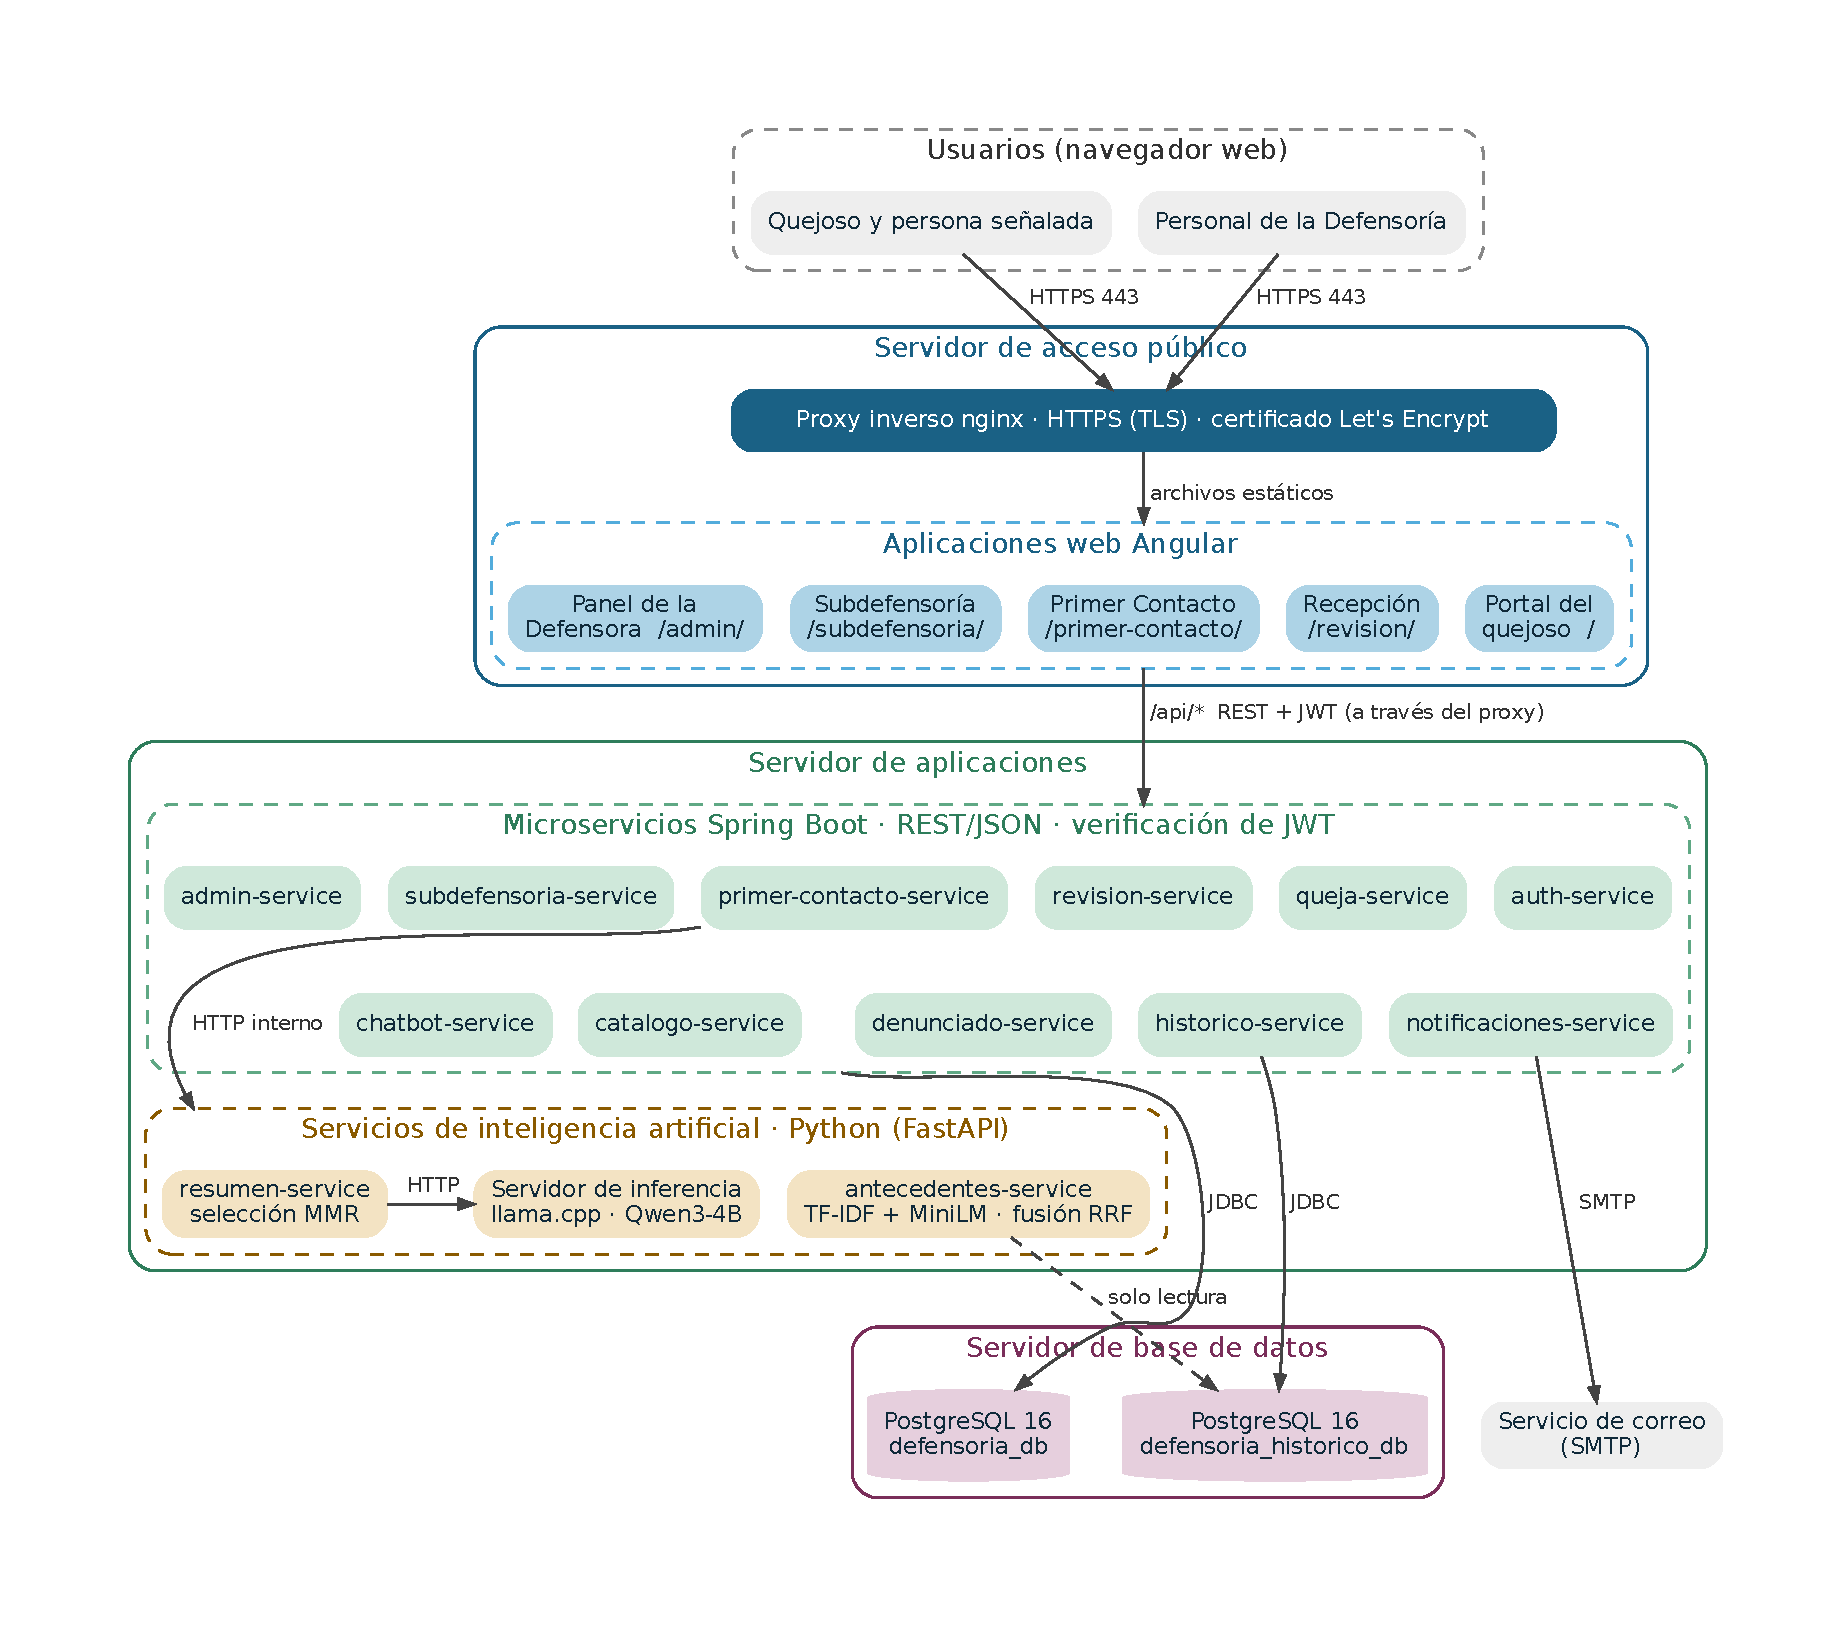
\includegraphics[width=0.82\textwidth]{arquitectura.pdf}
\caption{Arquitectura de la plataforma en tres servidores.}
\label{fig:arquitectura}
\end{figure*}

El servidor de aplicaciones aloja once microservicios desarrollados con Spring Boot, uno por responsabilidad del procedimiento (autenticación, quejas, Recepción, Primer Contacto, Subdefensoría, persona señalada, administración, notificaciones, catálogos, preguntas frecuentes y consulta histórica), que se comunican mediante REST y JSON. Aloja también tres servicios de inteligencia artificial en Python, accesibles solo desde la red interna: el de antecedentes, el de resúmenes y un servidor de inferencia que ejecuta el modelo generativo con llama.cpp. El servidor de base de datos contiene dos bases PostgreSQL~16: la operativa y la de quejas históricas. Cada servidor solo acepta conexiones del que le antecede.

La autenticación se basa en tokens JWT firmados: el servicio de autenticación emite los tokens de los quejosos y el de administración los del personal, mientras que el resto de los microservicios solo los verifica y autoriza cada operación según el rol (\texttt{RECEPCIONISTA}, \texttt{ANALISTA\_PRIMER\_CONTACTO}, \texttt{SUBDEFENSOR} o \texttt{DEFENSOR}). La elección de microservicios en lugar de una aplicación monolítica~\cite{villamizar} responde a tres razones: la separación de la información y las operaciones por área; el aislamiento de fallas, de modo que la caída del servicio de notificaciones o de los de inteligencia artificial no impide completar la operación principal; y el despliegue independiente de cada servicio en contenedores administrados con Podman, que además permite combinar Java y Python.

\subsection{Modelo de datos y ciclo de vida del expediente}

El esquema operativo consta de 29 tablas organizadas en cinco módulos: núcleo de quejas, Primer Contacto, persona señalada, Subdefensoría, y administración y catálogos. El expediente recorre tres tablas principales, una por etapa: \texttt{quejas} conserva la queja y su paso por Recepción; al turnarla se crea un registro en \texttt{expedientes\_primer\_contacto} que guarda el folio de la queja; y al dictaminarla como procedente se crea uno en \texttt{expedientes\_investigacion} que guarda el folio de Primer Contacto. Esta cadena de folios permite rastrear cada expediente desde su origen. Dentro de un servicio, las relaciones se declaran como llaves foráneas; entre servicios se usan referencias lógicas, verificadas en la lógica de negocio, para mantener independientes a los microservicios.

Cada etapa tiene estados definidos. En Recepción, la queja transita de \texttt{RECIBIDA} a \texttt{EN\_VALIDACION} y de ahí a \texttt{RECHAZADA} o \texttt{TURNADA}; en Primer Contacto, el expediente pasa de \texttt{TURNADA} a \texttt{EN\_ANALISIS} y concluye como \texttt{PROCEDENTE} o como \texttt{IMPROCEDENTE}, en cuyo caso se \texttt{REMITIDA} a la instancia competente; y en Subdefensoría avanza desde \texttt{RECIBIDO} por la investigación y la espera de los oficios hasta \texttt{CONCLUIDO}. Las reglas de negocio se validan en el servidor y no solo en la interfaz; por ejemplo, una queja solo es editable mientras está \texttt{RECIBIDA}, una queja solo puede ser tomada por una recepcionista a la vez, las citas de un analista no pueden empalmarse y un oficio sin respuesta antes de su fecha límite, calculada en días hábiles, cambia a \texttt{VENCIDO}.

\subsection{Recuperación híbrida de antecedentes}

A partir de la narrativa de una queja, el servicio de antecedentes recupera los expedientes vigentes e históricos más parecidos. La señal léxica se obtiene con TF-IDF sobre unigramas y bigramas~\cite{manning}, cuya forma general es
\begin{equation}
\text{tf-idf}(t,d,D)=\text{tf}(t,d)\cdot\log\frac{|D|}{\text{df}(t)},
\end{equation}
donde $\text{tf}(t,d)$ es la frecuencia del término $t$ en el documento $d$ y $\text{df}(t)$ el número de documentos de la colección $D$ que lo contienen. Los bigramas conservan expresiones como ``no autorizó'', cuyo sentido se pierde al separar las palabras. La señal semántica se obtiene con el codificador \texttt{paraphrase-multilingual-MiniLM-L12-v2}~\cite{reimers,minilm,hf_minilm}, que representa cada queja como un vector denso y permite relacionar narrativas redactadas con vocabulario distinto. En ambos casos, la cercanía entre una consulta $\mathbf{u}$ y un documento $\mathbf{v}$ se mide con la similitud coseno:
\begin{equation}
\text{sim}(\mathbf{u},\mathbf{v})=\frac{\mathbf{u}\cdot\mathbf{v}}{\lVert\mathbf{u}\rVert\,\lVert\mathbf{v}\rVert}.
\end{equation}

Como las puntuaciones de ambos recuperadores tienen escalas distintas, se combinan sus posiciones mediante \textit{Reciprocal Rank Fusion} (RRF) ponderada~\cite{rrf}:
\begin{equation}
\text{RRF}(d)=\sum_{r\in\mathcal{R}}\frac{w_r}{c+\text{rango}_r(d)},
\end{equation}
donde $\mathcal{R}$ es el conjunto de recuperadores, $w_r$ el peso de cada uno, $\text{rango}_r(d)$ la posición del documento en su lista y $c=60$ la constante de suavizado. Se fusionan los diez primeros candidatos de cada recuperador con una ponderación de 75\,\% para TF-IDF y 25\,\% para MiniLM. Las representaciones semánticas se almacenan en un índice persistente, de modo que solo se recalculan las de los documentos nuevos o modificados.

El resultado se presenta al analista de Primer Contacto como una lista ordenada de expedientes con su porcentaje de similitud (Fig.~\ref{fig:analisis_ia}). Las quejas con mayor similitud se señalan como posibles duplicidades, pero la decisión de vincular un antecedente corresponde al analista y queda registrada en el expediente.

\subsection{Generación de resúmenes}

El servicio de resúmenes opera en dos etapas. Primero, divide la narrativa en fragmentos y selecciona los más informativos con \textit{Maximal Marginal Relevance} (MMR)~\cite{mmr}, que en cada iteración elige el fragmento $s$ que maximiza
\begin{equation}
\text{MMR}(s)=\lambda\,\text{sim}(s,q)-(1-\lambda)\max_{s'\in S}\text{sim}(s,s'),
\end{equation}
donde $q$ es el texto de referencia, $S$ el conjunto de fragmentos ya seleccionados y $\lambda\in[0,1]$ regula el equilibrio entre relevancia y redundancia. Después, los fragmentos seleccionados se envían al modelo generativo Qwen3-4B-Instruct-2507~\cite{qwen3}, ejecutado en procesador central mediante llama.cpp, con instrucciones de redactar en tercera persona y conservar negaciones, actores y datos explícitos. La selección previa acota la entrada del modelo, pero introduce una limitación: un dato descartado por MMR ya no está disponible para la redacción.

El resumen se guarda junto con los fragmentos seleccionados y la versión del servicio que lo generó, y se muestra al analista como un borrador con indicador de revisión humana, acompañado de los fragmentos originales para su contraste (Fig.~\ref{fig:analisis_ia}).

\begin{figure}[t]
\centering
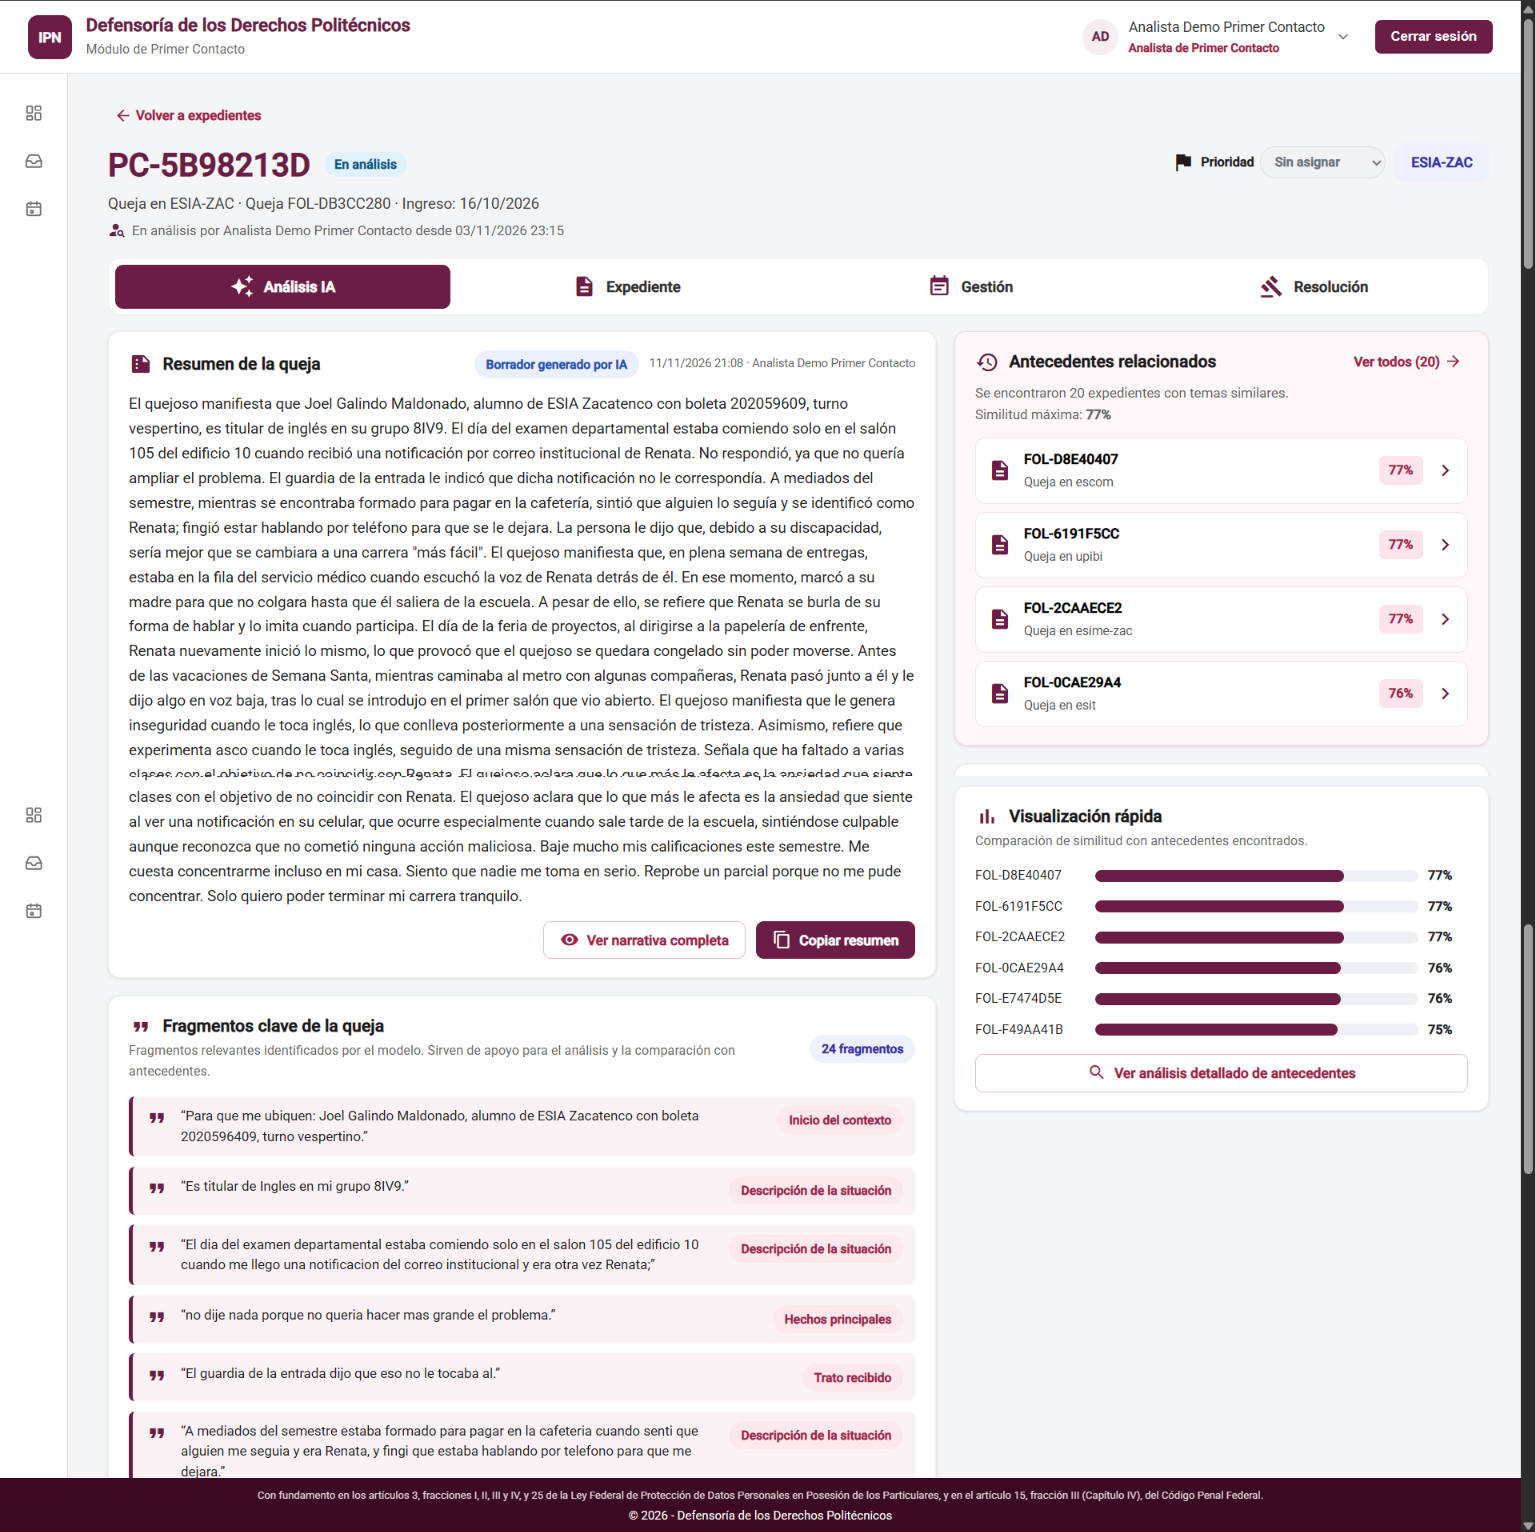
\includegraphics[width=\columnwidth]{analisis_ia_pantalla_completa.png}
\caption{Pantalla de análisis con inteligencia artificial en Primer Contacto: resumen generado, fragmentos clave y antecedentes relacionados con su similitud.}
\label{fig:analisis_ia}
\end{figure}

\subsection{Estrategia de pruebas}

Las pruebas siguieron el modelo en V~\cite{graham} y se organizaron según cinco atributos de calidad ---funcionalidad, robustez, fiabilidad, usabilidad y seguridad---, más una sección para los componentes de inteligencia artificial. Los datos de entrada se diseñaron con particiones de equivalencia, valores límite, tablas de decisión y transición de estados~\cite{myers}, y el esfuerzo se priorizó según el daño de cada falla: los accesos indebidos a datos personales, la ruptura del ciclo de estados y la atención simultánea de una queja se trataron como riesgos de máxima prioridad. Las pruebas unitarias se escribieron con JUnit~5 y Mockito, sustituyendo las dependencias por objetos simulados. En seguridad, un guion extrae del código la matriz de roles por punto de acceso y la compara con las reglas derivadas de los requerimientos. Para la usabilidad se fijó como criterio un puntaje SUS de al menos 68~\cite{brooke}.

Para el recuperador se emplearon dos conjuntos sintéticos. El primero contiene 200 quejas extensas, organizadas en 25 escenarios con ocho variantes de redacción cada uno; cada queja se usa como consulta y se consideran relevantes las de su mismo escenario. El segundo contiene 15 consultas contrastivas frente a 45 candidatos, con un antecedente relevante por consulta y documentos distractores. Se calcularon la precisión en los primeros cinco resultados (P@5), la exhaustividad en los primeros diez (R@10) y la ganancia acumulada descontada normalizada (nDCG@5)~\cite{manning}, y se recalculó la fusión sobre los rankings guardados para 101 ponderaciones, de 100\,\% léxico a 100\,\% semántico.

% =====================================================================
\section{Resultados}

\subsection{Pruebas funcionales, de robustez y de fiabilidad}

Se ejecutaron 364 pruebas unitarias sobre los diez microservicios Java de negocio, con 0 fallas y 0 errores (Tabla~\ref{tab:unitarias}). En las pruebas de integración se verificó que una queja turnada aparece en la bandeja de Primer Contacto, que el dictamen de procedencia crea el expediente en Subdefensoría y que el inicio de sesión unificado se comporta correctamente en siete escenarios. Se registraron por el formulario público 170 quejas sintéticas con credencial y evidencias. En robustez, el registro de la persona señalada rechazó las 19 entradas inválidas probadas y, en 10 intentos concurrentes de dos recepcionistas sobre la misma queja, no se produjo ninguna asignación doble. En fiabilidad, el dictamen se conserva y puede reenviarse cuando Subdefensoría no está disponible, y el resto de la plataforma siguió operando al detener contenedores auxiliares. Las cinco aplicaciones web compilan sin errores con la configuración de producción.

\begin{table}[t]
\caption{Pruebas unitarias por microservicio}
\label{tab:unitarias}
\centering
\renewcommand{\arraystretch}{1.15}
\begin{tabular}{|l|c|p{3.6cm}|}
\hline
\textbf{Servicio} & \textbf{Casos} & \textbf{Qué verifican} \\ \hline
queja-service & 112 & Validadores del registro, edición, conciliación \\ \hline
primer-contacto & 55 & Citas sin empalmes, dictamen, antecedentes \\ \hline
admin-service & 36 & Cuentas, bitácora, plantillas, respaldos \\ \hline
auth-service & 36 & Sesión, recuperación, contraseñas \\ \hline
revision-service & 36 & Toma atómica, turnado, historial \\ \hline
denunciado-service & 29 & Versión de la persona señalada \\ \hline
subdefensoria & 24 & Días hábiles, semáforo de plazos \\ \hline
notificaciones & 20 & Avisos e inyección de encabezados \\ \hline
catalogo-service & 8 & Importación tolerante a errores \\ \hline
chatbot-service & 8 & Preguntas frecuentes \\ \hline
\textbf{Total} & \textbf{364} & 0 fallas, 0 errores \\ \hline
\end{tabular}
\end{table}

\subsection{Pruebas de seguridad}

La matriz de permisos extraída del código abarcó 92 puntos de acceso, de los cuales 34 están regulados por los requerimientos. Su primera ejecución encontró seis diferencias; el análisis concluyó que el código reflejaba la decisión de diseño vigente, por lo que se corrigió la redacción de los requerimientos y no el código. Se verificó en el servidor que las rutas de Primer Contacto y Subdefensoría rechazan las peticiones sin token y que los puertos de los servicios y de la base de datos no son alcanzables desde Internet. Quedaron tres defectos abiertos: los secretos de configuración residen en texto plano en el repositorio (severidad alta), la descarga y restauración de respaldos no valida la ruta del archivo y la restauración sin confirmación responde con error 500 en lugar de 400 (severidad baja).

\subsection{Componentes de inteligencia artificial}

La Tabla~\ref{tab:rrf} resume la exploración de ponderaciones. En las 200 quejas extensas, la configuración adoptada de 75/25 alcanzó P@5 de 52.0\,\%, R@10 de 91.5\,\% y nDCG@5 de 0.490, a solo 0.3 puntos del mejor P@5 observado (90/10). En las consultas contrastivas, donde la coincidencia léxica es baja, la misma configuración obtuvo un R@10 de 13.3\,\%, mientras que las ponderaciones con predominio semántico alcanzaron 93.3\,\%. Los resultados evidencian un compromiso entre ambas señales y no una ponderación universalmente óptima; la configuración elegida puede omitir antecedentes descritos con paráfrasis complejas, por lo que la revisión humana es indispensable. Cabe señalar que en el conjunto contrastivo el valor máximo teórico de P@5 es 20\,\%, por lo que sus porcentajes no son comparables con los del primer conjunto.

\begin{table}[t]
\caption{Recuperación de antecedentes por ponderación TF-IDF/MiniLM}
\label{tab:rrf}
\centering
\renewcommand{\arraystretch}{1.15}
\begin{tabular}{|c|c|c|c|}
\hline
\textbf{TF-IDF / MiniLM} & \textbf{P@5} & \textbf{R@10} & \textbf{nDCG@5} \\ \hline
\multicolumn{4}{|c|}{\textit{200 quejas sintéticas extensas}} \\ \hline
100\,\% / 0\,\% & 45.2\,\% & 91.5\,\% & 0.435 \\ \hline
90\,\% / 10\,\% & 52.3\,\% & 91.5\,\% & 0.496 \\ \hline
\textbf{75\,\% / 25\,\%} & \textbf{52.0\,\%} & \textbf{91.5\,\%} & \textbf{0.490} \\ \hline
50\,\% / 50\,\% & 49.7\,\% & 67.5\,\% & 0.471 \\ \hline
25\,\% / 75\,\% & 48.5\,\% & 46.5\,\% & 0.457 \\ \hline
0\,\% / 100\,\% & 33.5\,\% & 46.5\,\% & 0.325 \\ \hline
\multicolumn{4}{|c|}{\textit{15 consultas sintéticas contrastivas}} \\ \hline
90\,\% / 10\,\% & 2.7\,\% & 13.3\,\% & 0.084 \\ \hline
\textbf{75\,\% / 25\,\%} & \textbf{2.7\,\%} & \textbf{13.3\,\%} & \textbf{0.084} \\ \hline
50\,\% / 50\,\% & 9.3\,\% & 86.7\,\% & 0.216 \\ \hline
25\,\% / 75\,\% & 9.3\,\% & 93.3\,\% & 0.219 \\ \hline
0\,\% / 100\,\% & 17.3\,\% & 93.3\,\% & 0.669 \\ \hline
\end{tabular}
\end{table}

En el servidor se verificó la construcción del índice sobre 1\,210 registros; una actualización sin cambios en los documentos reutilizó las 1\,210 representaciones almacenadas sin recalcularlas. Las consultas de antecedentes respondieron en aproximadamente 0.11 a 0.14~s, como observaciones puntuales y no como percentiles de latencia.

Una solicitud sintética al servicio de resúmenes respondió correctamente en 26.3~s. El borrador conservó las referencias a los correos y capturas del sistema y la negación de una agresión física, pero omitió dos fechas explícitas y un cambio de calificación de ocho a seis. Con la evidencia disponible no fue posible atribuir esas omisiones a la selección con MMR o a la redacción con Qwen3, por lo que se trata de una observación cualitativa de un caso y no de una tasa de fidelidad.

\subsection{Usabilidad}

Las sesiones de revisión con el personal de la Defensoría produjeron cambios concretos en la redacción jurídica de los requisitos de admisión, en la validación de Recepción y en el diseño de los paneles de Primer Contacto y de la Defensora, lo que equivale a varias iteraciones de prueba de usabilidad informal. La medición formal con el cuestionario SUS y las tareas cronometradas quedaron pendientes de la sesión de aceptación con la Defensoría.

% =====================================================================
\section{Conclusiones}

Se desarrolló y desplegó una plataforma web basada en microservicios que digitaliza el procedimiento de atención de quejas de la Defensoría de los Derechos Politécnicos, desde la presentación de la queja hasta la conclusión del expediente. La plataforma ofrece una solución técnica para cada problema identificado: el registro y la consulta de los expedientes se realizan en un mismo sistema; las narrativas extensas cuentan con resúmenes de apoyo; la búsqueda de antecedentes y de posibles duplicidades ya no requiere revisar manualmente los expedientes en papel; el estado de cada queja y sus plazos pueden consultarse en un solo lugar, tanto por el personal como por el quejoso; y la información de cada expediente pasa completa de un área a otra.

El objetivo de apoyar la clasificación de las quejas mediante PLN se redefinió durante el desarrollo: al analizar el dominio se concluyó que la determinación de la competencia es una decisión jurídica que no debe automatizarse, por lo que los componentes de inteligencia artificial se orientaron a apoyar el análisis previo a esa decisión. Con quejas sintéticas, el modelo de antecedentes alcanzó una precisión de 52\,\% en los primeros cinco resultados, pero un desempeño bajo ante paráfrasis complejas, y en los resúmenes se observaron omisiones de hechos. Ambos componentes deben considerarse herramientas de apoyo cuyo desempeño institucional aún debe confirmarse.

No puede afirmarse todavía que la ineficiencia del procedimiento esté resuelta en la práctica: para demostrarlo hace falta que la Defensoría opere la plataforma con quejas reales y que se mida la reducción en los tiempos de atención. Como trabajo a futuro se plantea validar los componentes de inteligencia artificial con expedientes reales y con criterios acordados con el personal, evaluando por separado las etapas de selección y de redacción de los resúmenes; reducir la latencia del modelo generativo mediante aceleración gráfica o generación en segundo plano; aplicar las pruebas de aceptación con el cuestionario SUS; retirar los secretos del repositorio antes de operar con información real; sustituir la creación automática del esquema por migraciones versionadas; e integrar la plataforma con los sistemas de identidad del Instituto.

Finalmente, el proyecto mostró que, ante una disponibilidad limitada de retroalimentación institucional, un desarrollo incremental con prototipos evolutivos permite que cada sesión con el cliente se traduzca en cambios concretos y que el sistema final responda al procedimiento real y no solo al descrito en los documentos.

% =====================================================================
\section*{Reconocimientos}

Los autores agradecen a la Escuela Superior de Cómputo del Instituto Politécnico Nacional por el apoyo recibido y las facilidades otorgadas para el desarrollo del presente trabajo terminal, así como al personal de la Defensoría de los Derechos Politécnicos por su participación en el levantamiento de requerimientos y en la revisión de los prototipos.

% =====================================================================
\begin{thebibliography}{99}

\bibitem{ipn_ley}
Instituto Politécnico Nacional, ``Ley Orgánica del Instituto Politécnico Nacional.'' [En línea]. Disponible: \url{https://www.ipn.mx/assets/files/defensoria/docs/manuales/ley-org\%C3\%A1nica-ipn.pdf}

\bibitem{ipn_acuerdo622}
Instituto Politécnico Nacional, ``Acuerdo de creación de la Defensoría de los Derechos Politécnicos,'' \emph{Gaceta Politécnica}, núm. 622 (Extraordinaria), pp. 3--7, ene. 2006.

\bibitem{ipn_mo_ddp}
Instituto Politécnico Nacional, \emph{Manual de Organización de la Defensoría de los Derechos Politécnicos}. Ciudad de México: Dirección de Planeación y Organización, 2022.

\bibitem{ipn_mp_ddp}
Instituto Politécnico Nacional, \emph{Manual de Procedimientos de la Defensoría de los Derechos Politécnicos}. Ciudad de México: Dirección de Planeación y Organización, 2024.

\bibitem{sidec}
Secretaría de la Función Pública, ``Sistema Integral de Denuncias Ciudadanas (SIDEC).'' [En línea]. Disponible: \url{https://sidec.buengobierno.gob.mx/}

\bibitem{eqs}
EQS Group, ``EQS Integrity Line.'' [En línea]. Disponible: \url{https://www.eqs.com/es/soluciones-gobierno-corporativo/integrity-line/}

\bibitem{unam_ddu}
Universidad Nacional Autónoma de México, ``Sistema de Denuncia en Línea de la Defensoría de los Derechos Universitarios.'' [En línea]. Disponible: \url{https://www.defensoria.unam.mx/denuncia/}

\bibitem{jurafsky}
D. Jurafsky y J. H. Martin, \emph{Speech and Language Processing}, 3a ed. (borrador en línea), 2026. [En línea]. Disponible: \url{https://web.stanford.edu/~jurafsky/slp3/}

\bibitem{villamizar}
M. Villamizar \emph{et al.}, ``Evaluating the monolithic and the microservice architecture pattern to deploy web applications in the cloud,'' Universidad de los Andes, Colombia.

\bibitem{pressman}
R. S. Pressman y B. R. Maxim, \emph{Software Engineering: A Practitioner's Approach}, 8a ed. New York: McGraw-Hill Education, 2014.

\bibitem{sommerville}
I. Sommerville, \emph{Software Engineering}, 10a ed. Boston: Pearson, 2016.

\bibitem{manning}
C. D. Manning, P. Raghavan y H. Schütze, \emph{Introduction to Information Retrieval}. Cambridge: Cambridge University Press, 2008.

\bibitem{reimers}
N. Reimers e I. Gurevych, ``Sentence-BERT: Sentence embeddings using Siamese BERT-networks,'' en \emph{Proc. EMNLP-IJCNLP}, Hong Kong, 2019, pp. 3982--3992.

\bibitem{minilm}
W. Wang, F. Wei, L. Dong, H. Bao, N. Yang y M. Zhou, ``MiniLM: Deep self-attention distillation for task-agnostic compression of pre-trained Transformers,'' en \emph{Advances in Neural Information Processing Systems}, vol. 33, 2020, pp. 5776--5788.

\bibitem{hf_minilm}
Sentence Transformers, ``paraphrase-multilingual-MiniLM-L12-v2,'' Hugging Face. [En línea]. Disponible: \url{https://huggingface.co/sentence-transformers/paraphrase-multilingual-MiniLM-L12-v2}

\bibitem{rrf}
G. V. Cormack, C. L. A. Clarke y S. Buettcher, ``Reciprocal rank fusion outperforms Condorcet and individual rank learning methods,'' en \emph{Proc. 32nd Int. ACM SIGIR Conf.}, 2009, pp. 758--759.

\bibitem{mmr}
J. Carbonell y J. Goldstein, ``The use of MMR, diversity-based reranking for reordering documents and producing summaries,'' en \emph{Proc. 21st Int. ACM SIGIR Conf.}, 1998, pp. 335--336.

\bibitem{qwen3}
Qwen, ``Qwen3-4B-Instruct-2507,'' Hugging Face. [En línea]. Disponible: \url{https://huggingface.co/Qwen/Qwen3-4B-Instruct-2507}

\bibitem{graham}
D. Graham, R. Black y E. van Veenendaal, \emph{Foundations of Software Testing: ISTQB Certification}, 4a ed. Andover: Cengage Learning, 2019.

\bibitem{myers}
G. J. Myers, C. Sandler y T. Badgett, \emph{The Art of Software Testing}, 3a ed. Hoboken, NJ: John Wiley \& Sons, 2011.

\bibitem{brooke}
J. Brooke, ``SUS: A `quick and dirty' usability scale,'' en \emph{Usability Evaluation in Industry}, P. W. Jordan \emph{et al.}, eds. Londres: Taylor \& Francis, 1996, pp. 189--194.

\end{thebibliography}

\end{document}
